\documentclass[a4paper]{article}

\usepackage[english]{babel}
\usepackage[utf8]{inputenc}
\usepackage{amsmath}
\usepackage{graphicx}
\usepackage{listings}
\usepackage{algorithmic}
\usepackage[ruled]{algorithm2e} % For algorithms
\usepackage[colorinlistoftodos]{todonotes}
\usepackage[inline]{enumitem}
\title{Final Multi-Agents System report}
\author{Emma Machielse, Federico Tavella, Alessandro Tezza}
\date{\today}

\begin{document}

\maketitle

\todo[inline]{max 10 pages. \textbf{readability}; grammar, syntax, scientific style, reference fig and tables.\textbf{ completeness}; what is done, why and the results, motivation design choice, how does system work}

\section{Introduction}
Public transport is an universal subject of travellers' complaints, targeted at the waiting and travel time. Attempts of transportation companies to reduce costs often have a detrimental effect on travelling time. A network of intelligent autonomous transportation units could optimize for lowering costs and travelling time. To illustrate this, a multi-agents system is created for an intelligent bus transport in Amsterdam. The goal of this system is to transfer passengers as efficient as possible. Several methods stated in game theory \cite{intromultiagentsystems} are implemented to create this system, like communication between buses, coordination and negotiation. 

\section{Framework}

We chose to organise our system using a Belief-Intention architecture, similar to the BDI one\cite{caillou2017simple}. In fact, every agent has a set of intentions, i.e.,  a set of tasks that it wants to achieve. Based on the state of the environment in a specific time (stored in the Beliefs and in some agent local variable), the agent choose the best intention to accomplish for that specific time. Intentions are future directed and trigger certain actions \cite{multiagentsystems}. This framework facilitates flexibility in generating actions, because an agent can switch between intentions depending on the state of the environment. 

The bus interests are shared between the fleet: every bus wants to minimize the costs, the average travelling time of the passengers and the number of messages sent. However, there are some cases in which the agents compete between each others to obtain a resource, as we will describe later.

The cooperation and competition behaviour are generally achieved through communication: different agents can send messages to each others. A message is formalized through the use of an ontology, for which the string of the message is splitted in a \textit{message type} and in a \textit{message content}, as follow:

\begin{verbatim}
"message_type message_content"
\end{verbatim}

For example, it is possible to ask to a bus to drive according to a specific schedule by sending it the following message:

\begin{verbatim}
"schedule 2"
\end{verbatim}

where 2 is the ID of the schedule.

\section{Conceptual description and strategy}
This section explains the various agent concepts used, how they are designed and implemented, and along which strategies. Four types of costs shape our strategies, the amount of money spend, the average waiting time, the amount of messages send, and the amount of people waiting. Costs arise by traveling and buying more buses. To reduce costs, the buses need to transport travelers efficiently. The more passengers they can transport in the shortest amount of time, the lower the costs will be.

\subsection{transportation and coordination}
Buses are allowed to travel according to a specific route. This route describes the connections between different bus stops. In the following paragraphs, we will focus on how we chose the different schedules and how the buses are traveling through them.
 
\paragraph{different fixed schedules}
In order to reduce the amount of time a passenger spends in a bus, the map is split into four different areas. They can be classified under the labels "West", "North", "Center" and "East". Thus, each area defines the set of bus stops composing a schedule.

Splitting the bus stops has two advantageous effects. A bus focuses only in its specific area: thus, it has to complete a shorter distance before passing the same stop again, so waiting time will be reduced. The time that a traveler spends in the bus will be shorter, which will reduce chances of buses being full and unable to pick up other travelers.

This solution does occasionally require transferring passengers from one area to another. This reduces the advantageous effects. Transfer passengers will have to wait at two bus stops before reaching their destination. To enable transportation of people between bus stops in different schedules, we defined the concept of \textit{joint position}. A \textit{joint position} is a bus stop that is shared between different areas. Thus, if \textit{bus stop 4} is shared between \textit{area 1} and \textit{area 2}, we say that \textit{bus stop 4} is a \textit{joint position}  between \textit{area 1} and \textit{2}. Stop 3 (\texttt{Centraal}), is a shared stop for all four areas. As a result, when a passenger that needs to change area in order to reach his destination is picked up, the bus will consider as the passenger destination the nearest \textit{joint position} with the desired area: the agent will bring the passenger there and it will drop it; then, an agent from the destination area will picked up the passenger from the \textit{joint position} and it will bring the passenger to his real destination. In order to avoid useless movements of passenger, we define some conditions to pick up a passenger from a bus stop:

\begin{enumerate}
\item the passenger destination is in the bus area, \textbf{or}
\item the passenger destination is not in the bus area \textbf{and} the passenger is not already in a \textit{joint position} with the destination area.
\end{enumerate}


\paragraph{Direction-based pick up}
Within an area, we define two different schedules. The first one is a route through all the bus stops of the area, the second one is the reverse of the first one. Thus, we can have bus travelling in the same area but following two different directions. Thus, we improved the travelling time by moving passengers along the direction that is faster in order to reach the destination. This adds a new condition to check whether a bus should pick from a stop to the ones listed in the previous paragraph: the passenger has to be picked up only if it is faster to move the passenger to the destination (or to the \textit{joint position}) using the bus schedule, compared to the opposite one. If this condition does not hold, the passenger will not be picked up, and he will wait for another bus that is travelling with the opposite schedule. This increases transportation efficiency, since buses carry passengers for a shorter amount of time and are thus able to carry more passengers. 

The number of buses assigned to areas and schedules is distributed based on the needs of that specific schedule, as we will explain later. In this way, schedule with higher need of buses will be provided with new buses.

\subsection{Roles}
\label{subsec:roles}
To ensure that the buses cooperate efficiently, they are assigned specific roles. Roles differ in their ancillary responsibilities and so a hierarchy of buses was created. 
\newline
Roles can also define the \textit{behaviour} of a bus. Using roles makes it easy to change the behaviour of a bus. 
\paragraph{Global coordinator}
A major responsibility is buying new buses, in case of shortage. If all buses would be able to, this would happen inefficiently and increase costs unnecessarily. Therefore only the first created bus with \texttt{ID = 24} is assigned this responsibility. This bus is on top of the hierarchy, and its role is defined as \textit{global coordinator}. 
\newline
The \textit{global coordinator} adds buses based on shortage. Shortage is defined as the difference between the total number of people waiting, and the total bus fleet capacity. The cheapest bus type that is able to manage the amount of waiting people, is added. Thus, when a shortage is experienced, the global coordinator will create new buses: as we will explain in the following, the newly created buses will be items of auctions in order to assign the bus to a specific schedule.

\paragraph{Local coordinators}
One step down in the hierarchy, are the \textit{local coordinators}. They are each responsible for one of the four areas in Amsterdam. Note that the \textit{global coordinator} is also a \textbf{local coordinator}. The \textit{global coordinator} is assigned to the "Centre", whereas the buses with \texttt{ID = 25, 26 and 27} are responsible for "West", "East" and "North" respectively. The local coordinators keep track of their area, by listing the buses assigned to their area, their fleet capacity and the number of people waiting. When a new bus is created, all the local coordinators compete between each other to assign the new bus in their area, as described in Section \ref{subsec:negotiations}.

\paragraph{Scouts}
Less important than the local coordinators are the \textit{scouts}. Note that the global coordinator and the local coordinators are also scout. The scouts are created at the beginning of the simulation: each schedule will have one scout. Their aim is to ensure that a bus in a specific schedule always exists. They do not have specific responsibility, but the semantic of the role specifies that they can not be moved from their schedule. 

\paragraph{Simple}
Finally, at the bottom of the hierarchy we have the simple buses. Every bus is also a simple bus. However, the bus created after the beginning of the simulation are \textbf{only} simple. This means that they do not have specific things to do, but they only have to pick, move and drop passengers. 

\subsection{Communication}
As stated before, to enable social interaction between agents with conflicting or agreeable goals, a form of communication is implemented. This communication happens through the exchange of messages. A bus sends a message with a specific goal, and the receiver performs actions based on the content.
\paragraph{Ontology}
To take into account the possibility of messages with different purpose, we defined the following ontology for communication: \texttt{"message\_type content"}. Where  \texttt{message\_type} is the header of the message, or the performative \cite{fipa}. This is a string that describes the goal of the message. Then \texttt{content} contains the effective content of the message. We implemented this ontology, so that buses know how to use the content of the message for, based on the performative. The perfomatives of the messages can be promoting, assigning, requesting help, offering help, accepting help, requesting a bid, bidding and reallocating. 
\newline
The reception of the messages goes as following. At every tick a bus checks its incoming messages. It can retrieve the new messages from the inbox history. To check whether a message is new, its tick is compared to the last tick at which the agent checked its inbox. This last tick is represented by a \textit{locally stored variable}. The performative of the message, implies how to interpret the content. Based on the content the bus could changes its intentions: for example, when a local coordinator gets a message of type ``\textit{bid-request}'', the new intention of performing the bid will be added.

\subsection{Group decisions}
The division of the route into four areas can lead to certain scenarios that involve unnecessary costs. Steps are taken to deal with a situation, where one area has a shortage of buses whereas the other area has a remnant. 

Local coordinators keep track of all the buses that move in their area. In addition, they compare the amount of people waiting in their area with the fleet capacity. Based on this comparison, they decide whether they need more buses. If this is the case, they collaborate with the other coordinators. 

This collaboration is done by sending a message to the other coordinators. The message has performative \textit{request help} and the content is a number; the shortage of fleet capacity. The other coordinators check if they have remnant buses, and if so send a message with performative \textit{offer help} and the content is the id of the bus that is remnant. Upon receiving this offer, the coordinator adds this bus to its bus fleet. A reply is send with performative \textit{accept help} and again as content the id of the offered bus. The other coordinator removes the bus from its bus fleet. The offered bus receives a message with performative \textit{reallocate} and the content contains the bus id of its new coordinator. Based on this new coordinator, the bus retrieves its new schedule. As soon as it reaches the transfer stop, it changes area. In this way, local coordinators from different areas can exchange buses between them. Thus, buses are distributed more efficiently and costs associated to the creation of new buses are reduced.

\subsection{Negotiation}
\label{subsec:negotiations}
The local coordinators compete between each others in order to obtain the newly created buses for their area.

When the global coordinator creates a new bus, it also sends a message ``\textit{bid-request}'' to every local coordinator, that will start the auction for the new bus. Every local coordinator will then send a message ``\textit{bid}'' to the local coordinator specifying the need of the two schedules in its area. The need for a specific schedule is computed counting the number of passengers in the area that should be picked up by a bus following the schedule (remember that based on the schedule, the direction of the bus changes, and passengers will be picked up based on the traveling direction). After receiving the bids from the local coordinators, the global coordinator will choose the schedule for which the need is higher, and it will specify to the newly created bus that it should drive using that schedule, sending it a message of type ``\textit{schedule}'' containing the ID of the schedule.

\subsection{Stopping buses}
\label{sec:stop}
We allow a bus to stop when some conditions are met. In this way, we can reduce the traveling costs when possible. In particular, a bus can stop when:

\begin{itemize}
\item the bus is empty \textbf{and}
\item there are no passengers waiting in its schedule; here, we consider the number of passengers waiting in the bus stops composing the schedule of the bus that have to be picked up (considering the direction of the bus).
\end{itemize}

However, as we will describe in Section \ref{sec:tuning}, not allowing the bus to stop brings to better results. Thus, we deactivated this feature.

\section{Code}
For clarity and readability, the code is divided in different files:

\begin{itemize}
\item the file agent implement the decision process of one agent: the management of beliefs and intentions;
\item the file init is used to initialized all the local variables of the agents;
\item the file execute-intentions implement the actions related to every intention;
\item the file messages implements some functions to interact with a message, for example the retrieval of the content of the message;
\item the file utils implements all the utility functions used by the other files.
\end{itemize} 

\section{Tuning}
The agent logic consists of a set of parameters that have been tuned for performance purposes. We tried different combinations of these parameters in the training set and in the two test sets, in order to find the best parameter setting. In particular, these parameters are:

\begin{itemize}
\item \textbf{stop}: whether we allow the bus to stop or not, as explained in Section \ref{sec:stop}; the tuning showed better results when we do not allow the buses to stop
\item \textbf{initial bus type}: the type of the buses created at the beginning of the simulation (the scout buses); we set this parameter to 3, i.e., the firstly created buses are red
\item \textbf{threshold for creating a new bus}: as we described in Section \ref{subsec:roles}, the global coordinator creates a new bus based on the shortage, i.e., the difference between the number of people waiting and the fleet capacity. The shortage is compared with this threshold: when the shortage is higher, new buses will be created; we set this parameter to 0, i.e., as soon as we have a shortage, we need to create new buses
\item \textbf{threshold for the bus types}: when the shortage is higher than the previous threshold, new buses will be created. The type of the newly created buses is determined by how much high is the shortage. Thus, we have three tresholds for the three bus types respectively; we set the threshold for creating a red bus to 60, the threshold for creating a yellow bus to 12 and the threshold for creating a blue bus to 0. This means that we create the cheapest bus that can ``manage'' the shortage situation. 
\end{itemize}

\section{Performance}

To establish the performance of the final code, a comparison is made to a baseline code. In the baseline code, buses only travel, pick up and drop off passengers, and create new buses. Table \ref{table:table1} shows that there is a significant decrease in the travel time and the amount of people waiting. In the final code, more buses are added which explains the increase in bus expenses. Also, the number of messages is increased, to enable cooperation between buses. 

\begin{table*}
\begin{tabular}{ |c|c|c|  }
 \hline
 \multicolumn{4}{|l|}{Table 1. Performance results} \\
 \hline
  Measurement & Baseline & Final Code \\
 \hline
  Avg travel time & 150 & 52 \\
  Buses' expenses & 1039682 & 5298614 \\
  Messages sent & 0 & 275  \\
  Final amount waiting & 232 & 25 \\
  Avg travel time remaining & 100 & 39 \\
  Final avg travel time & 156 & 54 \\
 \hline
\label{table:table1}
\end{tabular}
\end{table*}


From figure \ref{fig:pass_waiting} can be gathered that there is a peek in the number of passengers waiting during the morning rush hours. This peek lowers, when more buses are added. Thanks to the enlarged bus fleet, a much smaller peek is seen during the second rush hour in the evening.

See figure \ref{fig:expense}
see figure \ref{fig:messages}
See figure \ref{fig:avg_tt}

\begin{figure}
\centering
\begin{minipage}{.5\textwidth}
  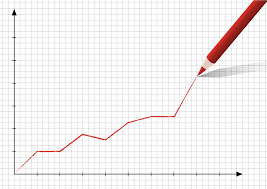
\includegraphics[width=.4\textwidth]{expenses.jpg}
  \caption{\label{fig:expense}Figure that displays the expenses of the buses.}
\end{minipage}%
\begin{minipage}{.5\textwidth}
  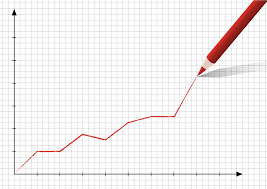
\includegraphics[width=.4\textwidth]{nr_messages.jpg}
  \caption{\label{fig:messages}Figure that displays the number of exchanged messages.}
\end{minipage}
\end{figure}

\begin{figure}
\centering
\begin{minipage}{.5\textwidth}
  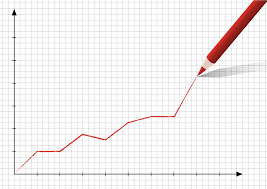
\includegraphics[width=.4\linewidth]{nr_pass_waiting.jpg}
  \caption{\label{fig:pass_waiting}Figure that displays the number of passengers waiting.}
\end{minipage}%
\begin{minipage}{.5\textwidth}
  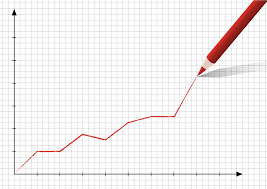
\includegraphics[width=.4\linewidth]{avg_tt.jpg}
  \caption{\label{fig:avg_tt}Figure that displays the average travelling time.}
\end{minipage}
\end{figure}

\section{Performance on test data}

Table 2 shows.


\begin{table*}
\begin{tabular}{ |c|c|c|  }
 \hline
 \multicolumn{4}{|l|}{Table 1. Performance results} \\
 \hline
  Measurement & Test Data set 2 & Test Data set 3 \\
 \hline
  Avg travel time & 0 & 0 & 0\\
  Buses' expenses & 0 & 0 & 0\\
  Messages sent & 0 & 0 & 0\\
  Final amount waiting & 0 & 0 & 0\\
  Avg travel time remaining & 0 & 0 & 0\\
  Final avg travel time & 0 & 0 & 0\\
 \hline
 \label{table:table2}
\end{tabular}
\end{table*}



\subsection{Conclusion}
From the results can be concluded that the number of passengers and the waiting time significantly decreased for each data set that is tested. The costs and the amount of messages did increase.

\section{Discussion}
Some implementations that could have led to better performance of the system are the following.
\newline
The amount of occupied spots in each bus is local information, that can only be made known to other buses through communication. This information could have been used to make a more accurate estimation of the amount of buses needed for the travellers. Since the current system is very sensitive to adding new buses, the information did not seem valuable. To reduce the amount of messages send, this information is not communicated.

\newpage
\onecolumn
\bibliographystyle{ieeetr}
\bibliography{bib}

\end{document}
